\documentclass[conference]{IEEEtran}
\IEEEoverridecommandlockouts
% The preceding line is only needed to identify funding in the first footnote. If that is unneeded, please comment it out.
\usepackage{cite}
\usepackage{amsmath,amssymb,amsfonts}
\usepackage{algorithmic}
\usepackage{graphicx}
\usepackage{textcomp}
\usepackage{xcolor}
\usepackage[brazilian]{babel}
\usepackage[utf8]{inputenc}
\usepackage[T1]{fontenc}
\usepackage{listings}
\usepackage{color}
\usepackage{float}
\usepackage{multirow}
\usepackage{hyperref}

\definecolor{dkgreen}{rgb}{0,0.6,0}
\definecolor{gray}{rgb}{0.5,0.5,0.5}
\definecolor{mauve}{rgb}{0.58,0,0.82}

\lstset{frame=tb,
  language=Java,
  aboveskip=3mm,
  belowskip=3mm,
  showstringspaces=false,
  columns=flexible,
  basicstyle={\small\ttfamily},
  numbers=none,
  numberstyle=\tiny\color{gray},
  keywordstyle=\color{blue},
  commentstyle=\color{dkgreen},
  stringstyle=\color{mauve},
  breaklines=true,
  breakatwhitespace=true,
  tabsize=3
}
\lstset{language=Python}
\def\BibTeX{{\rm B\kern-.05em{\sc i\kern-.025em b}\kern-.08em
    T\kern-.1667em\lower.7ex\hbox{E}\kern-.125emX}}
\begin{document}

\title{Relatório do Laboratório 10: \\ Detecção de objetos\\
}

\author{\IEEEauthorblockN{Isabelle Ferreira de Oliveira}
\IEEEauthorblockA{\textit{CT-213 - Engenharia da Computação 2020} \\
\textit{Instituto Tecnológico de Aeronáutica (ITA)}\\
São José dos Campos, Brasil \\
isabelle.ferreira3000@gmail.com}
}

\maketitle

\begin{abstract}
Esse relatório documenta a implementação de um algoritmo de detecção de objetos do futebol de robôs com base no algoritmo de YOLO (You Only Look Once), que por sua vez se baseia no uso de uma Rede Neural Convolucional (RNC).
\end{abstract}

\begin{IEEEkeywords}
\textit{YOLO}, Redes Neurais Convolucionais, Keras, Tensorflow
\end{IEEEkeywords}

\section{Implementação}
Para a implementação da rede neural conforme os parâmetros requisitados pelo roteiro do laboratório \cite{roteiro}, era necessário utilizar do código de adição de camadas a uma rede, fortemente inspirado das linhas de código apresentadas na seção Dicas do roteiro do laboratório \cite{roteiro}. Um detalhe importante a ser sitado foi que na criação das camadas de average pooling no Keras, os parâmetros \textit{px} e \textit{py} (no parâmetro \textit{pool\underline{\space}size}) são os tamanhos do Kernel apresentados nos requisitos para cada uma dessas camadas.

A rede então foi treinada utilizando o script \textit{train\underline{\space}lenet5.py} e os resultados desse treinamento foi exibido no \textit{Tensorboard}, mostrado a partir da execução do script \textit{run\underline{\space}tensorboard.py}. Ambos scripts já foram fornecidos previamente no código básico disponibilizado para esse laboratório.

Por fim, a rede foi avaliada no \textit{test set} usando o script \textit{evaluate\underline{\space}lenet5.py}, gerando exemplos gráficos de predições corretas e outras erradas.

\section{Resultados e Conclusões}

\subsection{Gráficos gerados no Tensorboard}
Uma amostra das imagens geradas pelo algorito de detecção de objetos YOLO foram reproduzidos nas Figuras de \ref{imagem1_detection} a \ref{imagem7_detection}. Por essas imagens consegue-se observar o correto funcionamento do algoritmo, indicando que a implementação foi feita corretamente. Assim como esperado, então, conseguiu-se detectar a bola e os postes das traves nas imagens fornecidas pelo professor.

\begin{figure}[htbp]
\centering
\centerline{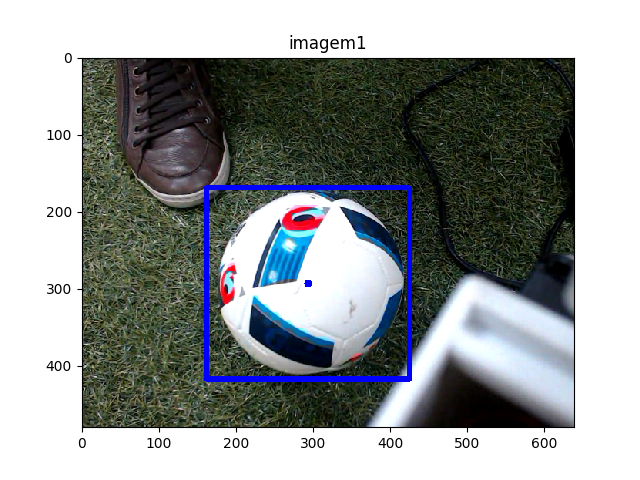
\includegraphics[scale=0.5]{imagens/imagem1_detection.png}}
\caption{Detecção de uma bola através do algoritmo de YOLO.}.
\label{imagem1_detection}
\end{figure}

\begin{figure}[htbp]
\centering
\centerline{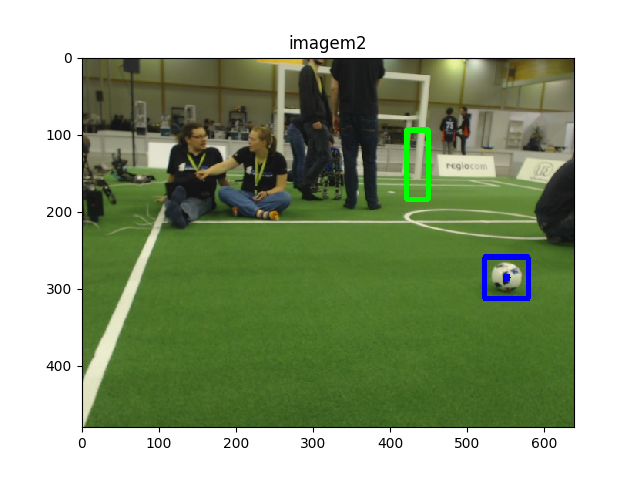
\includegraphics[scale=0.5]{imagens/imagem2_detection.png}}
\caption{Detecção de uma bola e de um dos postes da trave através do algoritmo de YOLO.}.
\label{imagem2_detection}
\end{figure}

\begin{figure}[htbp]
\centering
\centerline{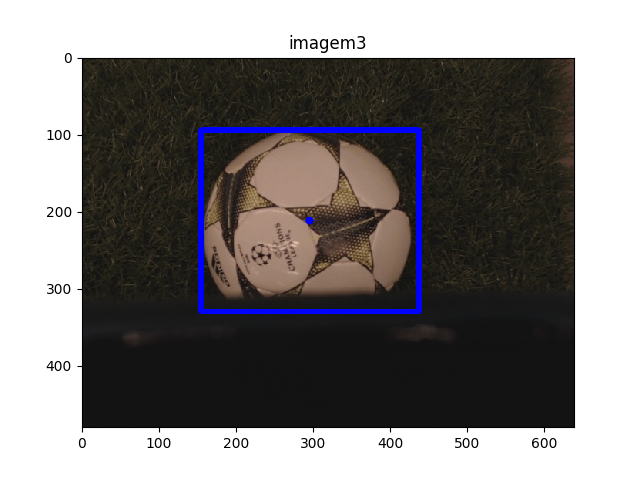
\includegraphics[scale=0.5]{imagens/imagem3_detection.png}}
\caption{Detecção de uma bola (mesmo que não completamente na imagem) através do algoritmo de YOLO.}.
\label{imagem3_detection}
\end{figure}

%\begin{figure}[htbp]
%\centering
%\centerline{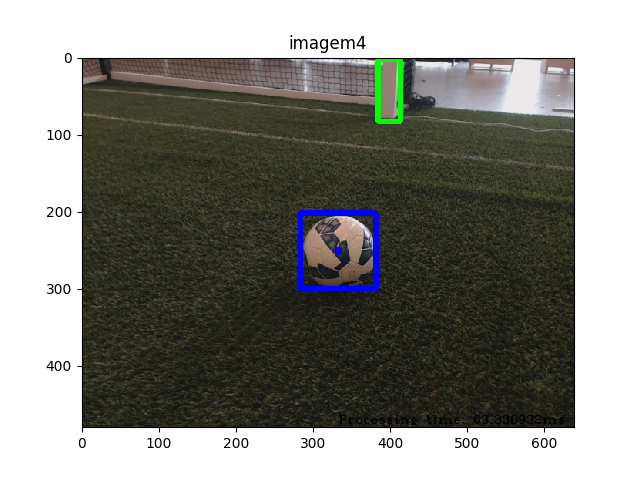
\includegraphics[scale=0.5]{imagens/imagem4_detection.png}}
%\caption{Custo do conjunto de validação, com o passar das épocas.}
%\label{imagem4_detection}
%\end{figure}

\subsection{Predições realizadas pela rede}
Após a implementação e treino da rede, avaliou-se os resultados da predição para novas entradas. Algumas imagens dos resultados foram apresentadas na Figura \ref{test_image_3758} para um número manuscrito corretamente predito, e na Figura \ref{misclassified_image_8} para uma predição incorreta. Chegou-se a uma acurácia de 0.9883 nesses casos testes.

Tendo em vista o que foi apresentado, pode-se notar, por fim, que a rede neural realmente se demonstrou eficaz em realizar essa predição de números manuscritos.

\begin{figure}[htbp]
\centering
\centerline{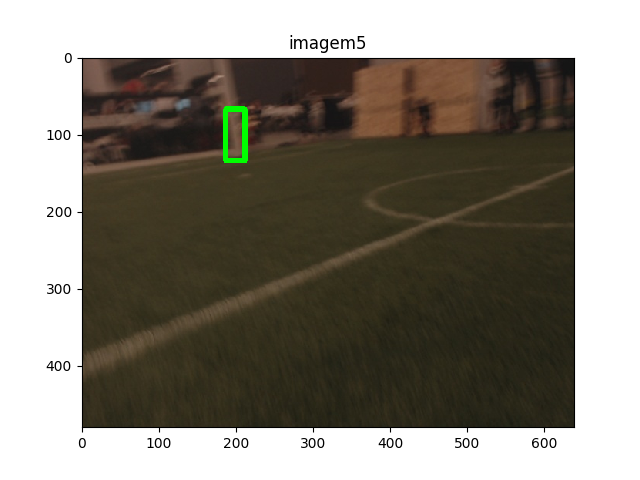
\includegraphics[scale=0.5]{imagens/imagem5_detection.png}}
\caption{Detecção de um poste de trave através do algoritmo de YOLO.}
\label{imagem5_detection}
\end{figure}

%\begin{figure}[htbp]
%\centering
%\centerline{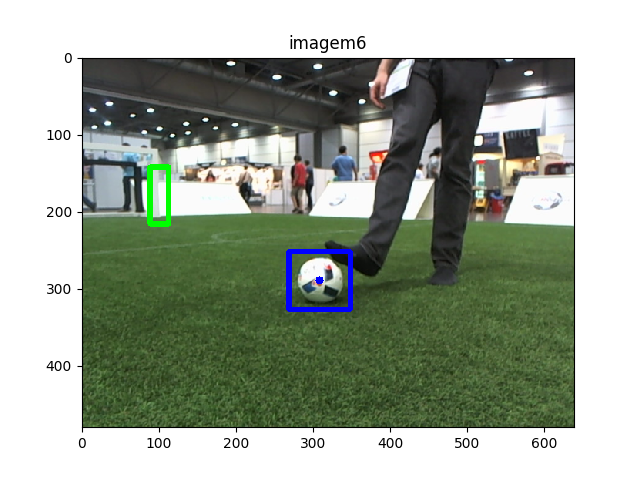
\includegraphics[scale=0.5]{imagens/imagem6_detection.png}}
%\caption{Número predito incorretamente.}
%\label{imagem6_detection}
%\end{figure}

\begin{figure}[htbp]
\centering
\centerline{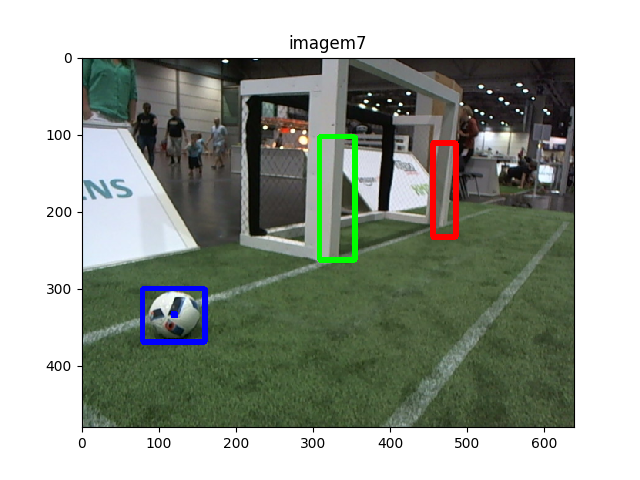
\includegraphics[scale=0.5]{imagens/imagem7_detection.png}}
\caption{Detecção de uma bola e dois postes da trave através do algoritmo de YOLO.}
\label{imagem7_detection}
\end{figure}

%\begin{figure}[htbp]
%\centering
%\centerline{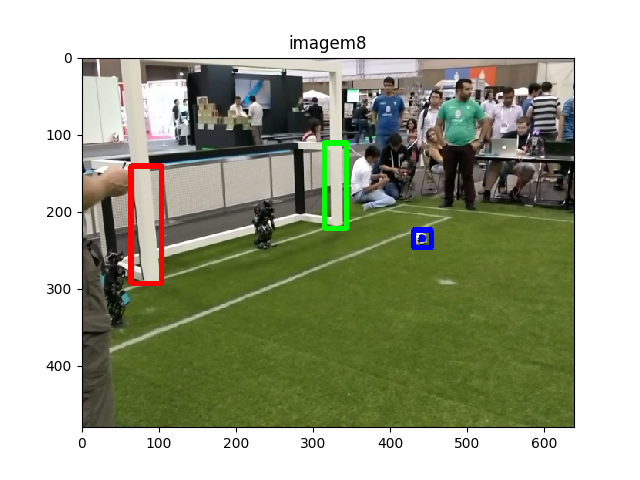
\includegraphics[scale=0.5]{imagens/imagem8_detection.png}}
%\caption{Número predito incorretamente.}
%\label{imagem8_detection}
%\end{figure}

%\begin{figure}[htbp]
%\centering
%\centerline{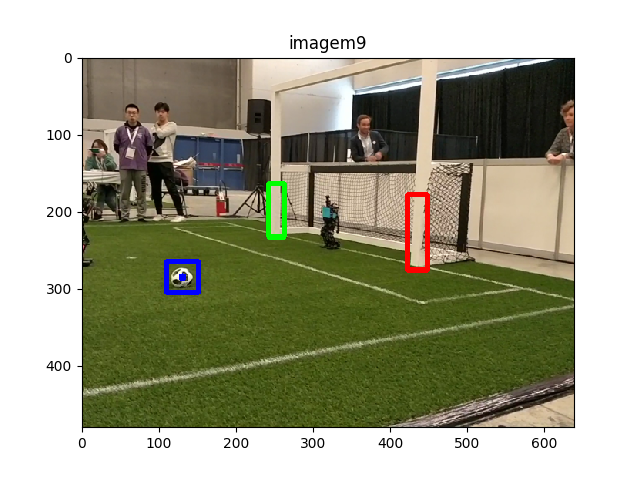
\includegraphics[scale=0.5]{imagens/imagem9_detection.png}}
%\caption{Número predito incorretamente.}
%\label{imagem9_detection}
%\end{figure}

%\begin{figure}[htbp]
%\centering
%\centerline{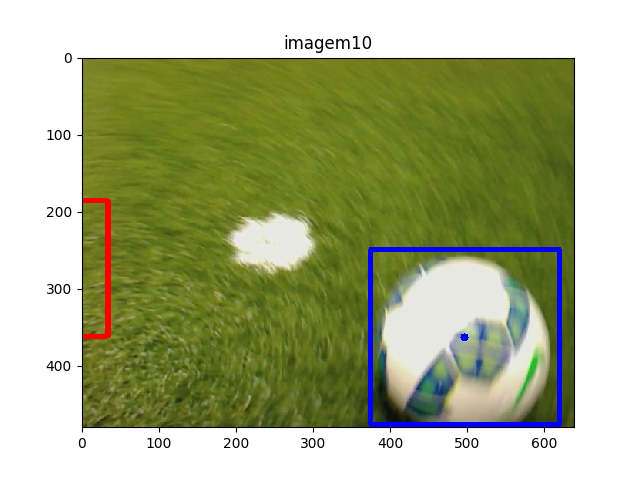
\includegraphics[scale=0.5]{imagens/imagem10_detection.png}}
%\caption{Número predito incorretamente.}
%\label{imagem10_detection}
%\end{figure}

\begin{thebibliography}{00}
\bibitem{roteiro} M. Maximo, ``Roteiro: Laboratório 10 - Detecção de Objetos''. Instituto Tecnológico de Aeronáutica, Departamento de Computação. CT-213, 2019.
\end{thebibliography}

\end{document}
